% \chapter{Theoretical Backgound}
\chapter{Fundamente teoretice}
În acest capitol se vor prezenta fundamentele teoretice proiectului, și se vor explica în detaliu deciziile architecturale luate în elaborarea proiectului.\newline
Scopul proiectului a fost proiectarea și implementarea unui program/sistem care este capabil să clasifice obiecte din imagini, să poată face detecția obictelor (adică să specifice unde se află acestea în imagine) și să facă segmentarea semantică a imaginii. Am ajuns la decizia că pentru aceste probleme o să folosesc o rețea neuronală convoluțională deoarece rețelele neuronale depășesc orice altă abordare capabilă să efectueze aceste sarcini.\newline
În primul rând o să se facă prezentarea rețelelor neuronale (convoluționale) și straturile specifice acestora. După aceasta vom afla cum se întâmplă antrenarea rețelei.




\section{Rețele Neuronale Convoluționale}
O rețea neuronală convoluțională - ca orice rețea neuronală - are la bază conceptul de \textit{neuron}, acesta fiind elementul din care se construiește. Aceștia sunt organizați în \textit{straturi de neuroni} (layer), straturile fiind interconectate formând o \textit{ierarhie de straturi}.\newline
Informația de intrare este alimentată \textit{stratului de intrare} (input layer). După aceasta semnaul se propagă printr-o serie de \textit{straturi ascunse}; în fiecare strat neuronii își calculează activarea prin folosirea \textit{funcției de activare}, iar activările se propagă în direcția \textit{stratului de ieșire} (output layer). Stratul de ieșire la rândul lui va furniza informația necesară (e.g. clasificarea obiectului din imagine, detecția obiectelor, segmentarea semantică, etc.).




\subsection{Neuronul Artificial}
În contextul științei biologiei neuronul este o celulă, un bloc de construcție, a cărui rol este colectarea semnalelor de la neuronii vecini prin dentriți, procesarea acestor informații, și pe baza informațiilor obținute și a structurii interne emite un semnal al lui prin axonul lui.\newline
%image of biological neuron
\begin{figure}[h!]
    	\centering
	\captionsetup{justification=centering, margin=2cm}
	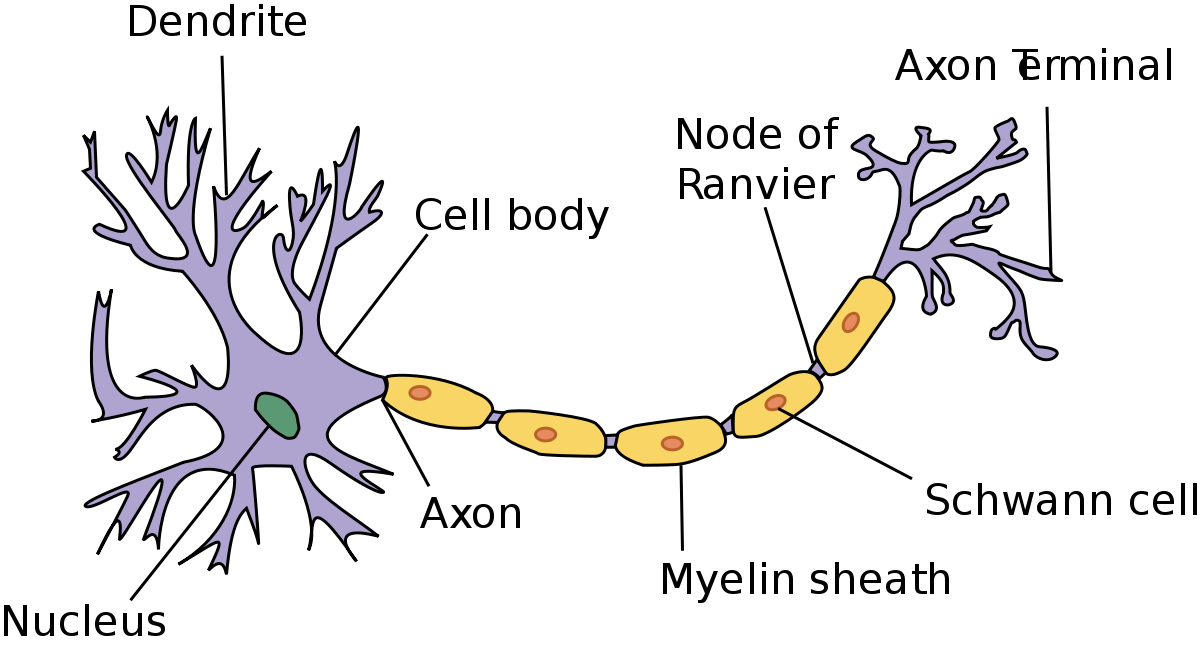
\includegraphics[width=0.5\textwidth]{figures/neuron.png}
	\caption{Neuronul - blocul de construcție a sistemului nervos \cite{neuron}}
	\label{fig:segmentare_semantica}
\end{figure}
Ideea neuronului artificial este bazată pe aceeași idee, părțile din care se compune fiind:
\begin{itemize}
	\item Intrările ponderate: semnalele/activările stratului anterior în șir sunt ponderate, asta însemnând că un neuron poate fi mai mult sau mai puțin influențat de un alt neuron. Ponderile sunt învățate în faza antrenării rețelei. Prin ponderi se introduce conceptul de \textit{neurons that fire together wire together}.
	\item Funcție de activare: pe baza intrărilor se calculează cât de tare este activat acest neuron.
	\item Ieșire: semnalul de activare se propagă la neuronii din stratul următor prin ieșirea lui.
\end{itemize}
%image of biological neuron
\begin{figure}[h!]
    	\centering
	\captionsetup{justification=centering, margin=2cm}
	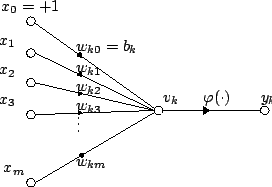
\includegraphics[width=0.5\textwidth]{figures/an.png}
	\caption{Modelul neuronului artificial \cite{arn}}
	\label{fig:neuronul_artificial}
\end{figure}

Neuronul biologic se activează (dă un semnal de ieșire) numai dacă semnalul de intrare depășește un anumit prag. În rețelele neuronale artificiale acest efect este simulat aplicând \textit{sumei ponderate} a intrărilor o fincție de transfer (activare) pentru a obține semnalul de ieșire.



\subsubsection{Descrierea matematică a funcționării unui neuron}
Întrările unui neuron se pot percepe ca o matrice de numere (fiecare fiind activarea unui neuron de pe stratul anterior) având $R$ elemente. Intrările individuale $p_1, p_2, \dots, p_R$ sunt înmulțite cu ponderile $w_{1,1}, w_{1,2}, \dots, w_{1,R},$ și valorile ponderate se însumează. Suma se poate nota cu \textbf{Wp}, adică produsul scalar al matricei \textbf{W} și vectorul \textbf{p}.\newline
Neuronul are \textit{ b (bias)}, care se adună cu intrările ponderate, rezultând arguentul $n$ al funcției de transfer
\begin{equation}
f: w_{1,1}p_1 + w_{1,2}p_2 + \dots + w_{1,R}p_R + b = n
\end{equation}
Această poate fi scrisă cu notația abreviată:
\begin{equation}
n = W*p + b; a = f(n)
\end{equation}


% enumerate the usual activation functions of neurons
Dacă ne uităm la funcțiile de transfer a neuronilor artificiali des folosite, vedem că există mai multe tipuri sau categorii de neuroni acestea fiind:
\begin{itemize}
	\item \textit{Threshlod neurons} (neuronii cu funcția treaptă): acest tip de neuron are cea mai simplă funcție de activare; ia intrările de la neuronii din stratul anterior, multiplică activările acestora cu ponderea respectivă pentru fiecare și calculează suma numerelor obținute după înmulțire. Înainte de a da ai departe rezultatul, se mai scade un număr special, numit \textit{bias}. Dacă rezultatul scăderii este mai mare decât zero, atunci ieșirea neuronului este unu, altfel zero.
\begin{equation}
	activation =
		\begin{cases}
			1, \text{if } n > 0 \\
			0, \text{otherwise}
		\end{cases}
\end{equation}
	\item \textit{Linear combination neuron} (neuronii cu funcția de transfer liniară - purelin): acest tip de neuron se comportă asemănător cu neuronii de prag. Ia intrările, calculează suma intrărilor ponderate și din această sumă scade bias-ul. Dacă rezultatul este mai mic decât zero, atunci activarea acestui neuron va fi zero. Între zero și unu, se propagă mai departe valoarea calculată. Peste unu, valoarea trimisă mai departe va fi și ea unu.
\begin{equation}
	activation = purelin(n)
\end{equation}
	\item \textit{Sigmoid neuron}:  neuronii care fac parte din această categorie folosessc o funcție non-liniară pentru a calcula activările lor: funcția sigmoidală. Această funcție este aleasă fiindcă calcularea derivativei ei este ușoară aceasta fiind a caracteristică crucială pentru a face posibilă antrenarea rețelei cu ajutorul algoritmului \textit{baskpropagation}.
\begin{equation}
	a = \frac{1}{1 + \mathrm{e}^{-n}}
\end{equation}
\end{itemize}

%image of biological neuron
\begin{figure}[h!]
    	\centering
	\captionsetup{justification=centering, margin=2cm}
	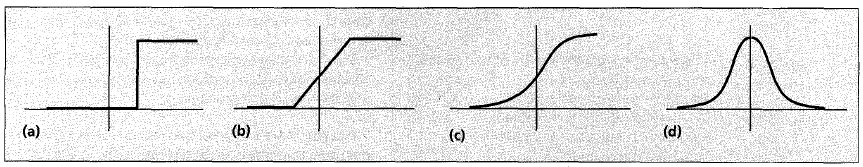
\includegraphics[width=0.7\textwidth]{figures/activation_functions.png}
	\caption{Funcții de transfer \cite{activationFunctions}}
	\label{fig:activationFunctions}
\end{figure}



\subsection{Rețeaua Neuronală Artificială}
Acum că am stabilit ce este un neuron artificial, categoriile neuronilor și funcționarea fiecăruia, putem lua un pas înapoi să vedem imaginea întreagă: rețeaua neuronală artificială care este construită din neuroni.\newline
Rețelele neuronale artificiale sunt utilizate pe scală largă în contextul inteligenței artificiale. Modelul și modul de funcționare a acestora este inspirată de modelul rețelelor neuronale din sistemul nervos al animalelor și al omului (imitând funcționarea sistemului nervos central sau a creierului).\newline
Popularitatea lor provine din faptul că acestea sunt capabile de a învăța funcți incredibil de complexe, cu mii de parametri (datoritp numărului mare de ponderi care pot fi învățate pentru a ajunge la o estimare cu ajustare precisă). Rețelel neuronale au urmâtoarele caracteristici importante:
\begin{itemize}
	\item Architectură: aceasta cuprinde decizii asupra numărului de straturi de neuroni, parametrii ca și numărul neuronilor pe fiecare strat aparte, ponderile conexiunilor, și inițializarea acestora.
	\item Regula de învățare/algoritmul de învățare: este mechanismul ales care va îndeplini sarcina ajustării ponderilor în fiecare iterație de antrenare. Alegerea algoritmului corespunzător este de o importanță crucială, și trebuie examinată pentru că un algoritm necorespunzător ar putea rezulta în incapabiliatea de a antrena rețeaua.
	\item Funcțiile de transfer a neuronilor din fiecare strat
\end{itemize}

% NeuNet with one hidden layer IMAGE
\begin{figure}[h!]
    	\centering
	\captionsetup{justification=centering, margin=2cm}
	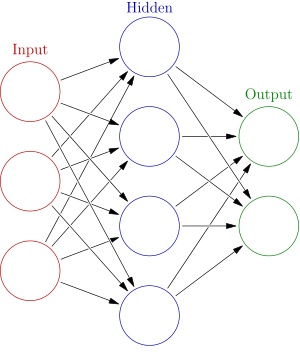
\includegraphics[width=0.3\textwidth]{figures/artificialneunet_1hidden.png}
	\caption{O rețea neuronală artificială cu un singur strat ascuns \cite{arn}}
	\label{fig:activationFunctions}
\end{figure}
Rețelele neuronale au o serie de straturi de neuroni, acestea de obicei fiind numerotate de la $L_0$ până la $L_N-1$ unde N este adâncimea rețelei neuronale. Neuronii de pe stratul $L_i$ primesc intrările de la stratul anterior, $L_i-1$. Folosind aceste intrări neuronul aplică funcția lui de transfer, rezultatul fiin activarea neuronului. Această activare se propagă mai departe spre stratul următor, adică $L_i+1$ unde va constitui parte din intrările neuronilor.


Între două straturi de neuroni vecini există $R*S$ ponderi, $R$ și $S$ fiind numărul neuronilor pe cele două straturi. De reguă aceste ponderi sunt organizate într-o matrice de ponderi:
\begin{equation}
	W = \begin{bmatrix}
		w_{1,1} && w_{1,2} && \dots && w_{1,R} \\
		w_{2,1} && w_{2,2} && \dots && w_{2,R} \\
		\dots && \dots && \dots && \dots\\
		w_{S,1} && w_{S,2} && \dots && w_{S, R} \\
	\end{bmatrix}
\end{equation}



\subsubsection{Rețele neuronale cu straturi multiple de neuroni}
O rețea neuronală artificială poate acea mai multe straturi, fiecare strat având o matrice a ponderilor \textbf{W}, un vector al deplasărilor \textbf{b} și un vector de ieșire \textbf{a}. Pentru a distinge matricile ponderilor, vectorii de ieșire, etc., pentru fiecare strat din rețea notăm numărul stratului ca superscript la variabila respectivă. O intrare constantă este atașată fiecărui neuron, asta fiindu-i \textit{deplasarea (bias)}. Ieșirile din fiecare strat intermediar reprezintă intrările pentru stratul următor. Astfel, stratul $i$ are $S^{i-1}$ intrări, $S^{i}$ neuroni și o matrice $W^2$ a ponderilor (cu dimensiunile $S^{i}\times S^{i-1}$). Intrarea in stratul $S^{i}$ este $a^{i-1}$, iar ieșirea este $a^{i}$. Această abordare se poate aplica oricărui strat din rețea.\newline
Straturile pot avea roluri diferite:
\begin{itemize}
	\item stratul care produce ieșirea rețelei este numit \textit{strat de ieșire}
	\item celelalte straturi se numesc \textit{straturi ascunse}
\end{itemize}
Ieșirea ultimului strat este ieșirea rețelei, și se notează cu $y$. Rețelele multi-strat sunt foarte eficiente. De obicei acestea au mai multe straturi ascunse cu neuroni sigmoidali, urmate de un strat de neuroni liniari. Fiindcă există mai multe straturi de neuroni cu funcție non-liniară de transfer, rețeaua este capabilă să învețe atât funcții liniare cât și funcții neliniare. Ultimul strat liniar permite rețelei să producă și rezultate care sunt în afara intervalului $[-1, 1]$.


\subsection{Antrenarea}
În această secțiune se va prezenta conceptul de \textit{machine learning} în contextul inteligenței artificiale, și cum învață rețelele neuronale (prin explicarea funcționării algoritmului de propagare inversă a erorii).\newline

\subsubsection{Machine Learning}
Este un domeniu a științei calculatoarelor care se ocupă cu algoritmi care cunt capabili de a generaliza, a învăța concepte care nu erau programate explicit. În această lucrare se folosesc rețele neuronale artificiale pentru a învăța concepte complexe precum recunoașterea obiectelor din imagini (mai particular se va vorbi despre învățarea supravegheată).

\paragraph{Metodele de învățare}


\subparagraph{Învățarea Supravegheată} \textit{(supervised learning)} presupune în orice moment (pentru orice set de date de intrare) existența unei valori dorite ($target$) pentru fiecare neuron din stratul de ieșire a rețelei. Sistemului i se furnizează seturi de perechi de intrare-ieșire dorită cu ajutorul cărora se calculează mrimi de eroare în funcție de diferența dintre valoarea reală a ieșirii și cea dorită, pe baza cărora se ajustează valorile parametrilor rețelei (interconexiuni și eventual valori de prag ale funcțiilor de activare). 


\subparagraph{Învățarea Nesupravegheată} \textit{(unsupervised learning)} rețeaua extrage singură anumite caracteristici importante a datelor de intrare formând reprezentări interne distincte ale acestora. Rețeaua nu beneficiază de seturi de ieșire dorite, în schimb se utilizează un gen de "competiție" între neuronii elementari care are ca efect modificarea conexiunilor aferente numai neuronului care "câștigă" întrecerea, restul legăturilor rămânând neafectate.


\subparagraph{Învățarea folosing un "critic"} \textit{(reinforcement learning)} este denumită uneori și cu recompensă/pedeapsă ($reward/punishment$). În această situație, rețeaua nu beneficiază de un semnal dorit ca în cazul învățării supravegheate, ci de un semnal care oferă o informație calitativă ilustrând cât de bine funcționează sistemul (informația este binară, de tipul "răspunsul este bun/greșit"). Algoritmii aparținând acestei categorii sunt inspirați într-o mai mare măsură de observații experimentale făcute pe animale și, în esență, funcționează după următorul principiu: dacă urmarea unei anumite acțiuni întreprinse de un sistem capabil să învețe are un efect favorabil, tendința de a produce acțiunea respectivă în situația respectivă este încurajată, în caz contrar este inhibitată.


\subsection{Antrenarea Rețelelor Neuronale}
După ce ponderile și deplasările rețelei au fost inițializate, rețeaua este pregătită pentru a fi antrenată. Procesul de antrenare necesită un set mare de valori privind comportarea rețelei: intrări in rețea $p$ și ținta ($target$) t. În timpul antrenării, ponderile și deplasările sunt ajustate iterativ pentru ca rețeaua neuronală să greșească cât mai puțin.\newline


\subsubsection{Funcția de cost} Funcția de cost este funcția folosită pentru specificarea erorii pe care a făcut rețeaua pentru un set dat de intrări-ieșiri dorite. Pentru fiecare stare a rețelei neuronale putem asigna o valoare numerică, cu care putem descrie eroarea. Această valoare se numește \textit{cost}.\newline
Cu cât costul este mai mare, cu atât rețeaua este mai departe de starea în care am dori să fie. Cum se micșoreză costul, așa rețeaua neuronală ajunge mai aproape de o configurație a parametrilor în care produce predicțiile pe care le-am dori. Valoarea costului este calculată de \textit{funcția de cost}. Zicem că un model este $optimal$ dacă nu putem găsi o altă asignare a valorilor parametrilor rețelei astfel încât să ne producă un cost mai mic.\newline
Cu toate aceste noțiuni explicate, putem formula ce ar însemna învățarea/antrenarea pentru rețele neuronale: antrenarea este procesul iterativ prin care în fieare iterație costul rețelei neuronale scade, asta însemnând că pas cu pas predicțiile rețelei ajung mai aproape de realitate. În fiecare iterație de antrenare vrem să modificăm valorile ponderilor interconexiunilor și valorilor deplasărilor astfel încât să scadă costul. Pentru a atinge acest scop, de regulă se folosește algoritmul numit $propagarea inversă a erorii$.


\subsubsection{Propagare Inversă și Metoda Gradientului Negativ}
Cea mai simplă interpretare a algoritmului de propagare inversă actualizează ponderile rețelei și deplasările în direcția în care funcția de performanță scade cel mai rapid, adică în direcția gradientului negativ.\newline
Dacă am avea o singură pondere într-o rețea, atunci optimizarea rețelei ar fi destul de simplă: am putea încerca toate valorile pentru ponderea respectivă și am putea alege valoarea cu care primim cel mai bun rezultat. Problema este că dacă numărul de ponderi este mai mare, atunci această abordare devine incredibil de ineficientă. Aici vine ideea vicleană a propagării inverse: nu suntem nevoiți să încercăm toate configurațiile de ponderi și deplasări; de fapt ajunge să le inițializăm la întâmplare, și după aceasta le actualizăm iterativ astfel încât în fiecare iterație să ajungem la un cost mai mic decât în iterația anterioară astfel ajungând la o soluție mai aproape de cea optimă.\newline


\paragraph{Descrierea matematică a metodei gradientului negativ}
Să fie $F(x)$ o funcție multi-variabilă, care se poate deriva în vecinătatea punctului $a$. Atunci, dacă vrem să aflăm setul variabilelor care care conduc spre minimul funcției, ar trebui să luăm un $pas$ din $a$ în direcția speficicată de gradientul negativ a funcției $F$ în punctul $a$:
\begin{equation}
	b = a - \gamma \nabla F(a).
\end{equation}
Acesta va asigura, că $F(b) < F(a)$ însemnând ca punctul $b$ este mai aproape de minimul funcției $F$.


%visualization of gradient descent
\begin{figure}[h!]
    	\centering
	\captionsetup{justification=centering, margin=2cm}
	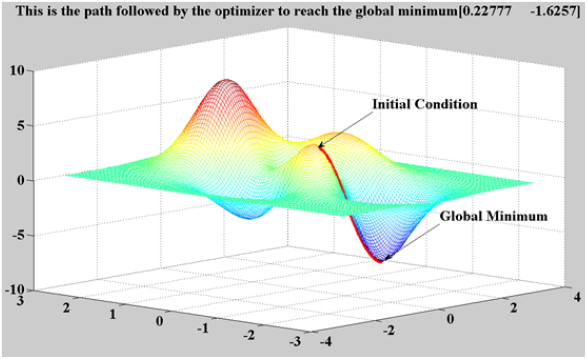
\includegraphics[width=0.9\textwidth]{figures/gradient_descent.png}
	\caption{Vizualizarea metodei gradientului negativ pentru o funcție cu două variabile \cite{arn}}
	\label{fig:gradient_descent}
\end{figure}

Repetând acest proces (calcularea gradientului în punctul curent, și actualizarea parametrilor prin scăderea gradientului), dacă pasul de învățare este destul de mic, atunci vom converga către un minim local. Dacă funcția $F$ este una convexă, atunci metoda gradientului invers ca converga către un punct foarte apropiat de minimul global.

\paragraph{Propagarea inversă}
Metoda propagării inverse a erorii este aplicată pe scală largă în domeniul rețelelor neuronale, la procesul de antrenare. Este folosit împreună cu metode de optimizare cum ar fi metoda gradientului negativ.\newline
Metoda constă din calcularea gradientului funcției de cost $C$, pentru fiecare pondere a rețelei neuronale. După ce gradientul funcției de cost este calculat, acesta este dat metodei de optimizare (gradient negativ), care pe baza gradientului actualizează ponderile interconexiunilor dintre neuroni și deplasările acestora. Astfel în fiecare iterație de antrenare, valoarea erorii este propagată dinspre stratul de ieșire către stratul de intrare, actualizând întreaga rețea.\newline
Această metodă de antrenare necesită un set de antrenare care conține atât exemple cât și predicția dorită pentru fiecare, pentru că folosind predicțiile dorite putem să calculăm eroarea (sau costul) rețelei pentru un set de intrări. Când antrenăm o rețea neuronală folosing propagarea inversă, evenimentele se pot separa în două faze:\newline

\subparagraph{Propagarea Înainte și Propagare Inversă} constituie propagarea activărilor neuronilor dinspre stratul de intrare către stratul de ieșire și propagarea inversă a erorii calculate de la stratul de ieșire spre stratul de intrare. Când semnalul ajunge la stratul de ieșire, se calculează diferența dintre predicția rețelei neuronale și \textit{target}-ul dorit. Pasul doi este propagarea acestei erori înapot, pentru a afla cum trebuie actualizate ponderile interconexiunilor și deplasările neuronilor.

\subparagraph{Weight Update} este faza în care se aplică următorii pași: înmulțim diferența fiecăruii nod cu semnalele de intrare; așa primim gradientul cu privire la ponderea conexiunii. În al doilea pas scădem o parte a gradientului punctului respectiv din ponderile nodului.\newline
\begin{equation}
	W \prime = W-\alpha \nabla ,
\end{equation}
unde $\alpha$ este rata de învățare (\textit{learning rate/learning speed}). Valoarea lui $\alpha$ se poate schimba dinamic între iterații de învățare, dar rămâne constant în timpul unei iterații. Valoarea și algoritmul de actualizare a ei trebuie aleasă cu mare grijă. Un $\alpha$ mai mare este echivalent cu luarea unor pași mai mari în jos, spre minimul funcției de cost/performanță. Acest lucru este dorit fiindcă rețeaua învață mai repede, dar are un dezavantaj foarte important: dacă pasul de învățare este una prea mare, atunci se poate întâmpla că pășim peste minimul suprafeței funcției de cost adică pășim peste soluția optimă fără să observăm. Pe de altă parte un $\alpha$ mai mic ne permite a să convergăm cu o acuratețe mai mare de soluția optimă, dar dezavantajul este că se poate bloca la fiecare minim local, nefiind capabil să iasă din punctele aparent bune (se poate opri la un punct foarte ne-optim pe suprafața de cost doar pentru că aceasta este un minim local.

\subsection{Date de Antrenare și Testare}
Antrenarea este faza în care rețeaua neuronală învață prin actualizarea ponderilor conexiunilor și actualizarea deplasărilor fiecărui neuron. Pentru a realiza antrenarea rețelei neuronale avem nevoie de un set de antrenare suficient de mare alcătuit din imagini etichetate (invățare supravegheată). Rețeaua neuronală face o predicție pe baza unei imagini din setul de antrenare, predicția fiindu-ne vizibilă la stratul de ieșire. Când eticheta ghicită de rețea apare la ieșire, calculăm un cost: diferența dintre predicția rețelei și valoarea adevărată, adică eticheta imaginei corespunzătoare. Având costul calculat suntem capabili să actualizăm ponderile și deplasările, astfel încât să-l micșorăm, folosing algoritmii prezentați mai sus. După o perioadă de antrenare (e.g. 1000 iterații de antrenare) avem o rețea neuronală a cărui ponderi sunt mai aproape de cele optimale decât parametrii rețelei nou-inițializate.\newline
Acum urmează pasul în care testăm cât de bine funcționează rețeaua neuronală. Avem la îndemână un set mare de imagini etichetate, care n-au fost folosite la antrenare. Comparăm predicțiile rețelei cu etichetele reale ale imaginilor și facem statistici privitoare la precizia predițiilor.


\section{Rețele Neuronale Convoluționale}
Rețelele neuronale convoluționale sunt un tip special a rețelelor neuronale, și s-au demonstrat foarte folositoare pentru recunoașterea, detecția și segmentarea imaginilor iar pentru analizarea semnalelor audio.\newline
Ele folosesc tipuri de straturi specifice rețelelor convoluționale.

\subsection{Straturi convoluționale}
Straturile convoluționale sunt alcătuite dintr-un set de filtre convoluționale (\textit{convolutional kernerls)}. După antrenarea rețelei astea devin niște filtre \textit{Gabor-like}.

%Gabor-like filters
\begin{figure}[h!]
    	\centering
	\captionsetup{justification=centering, margin=2cm}
	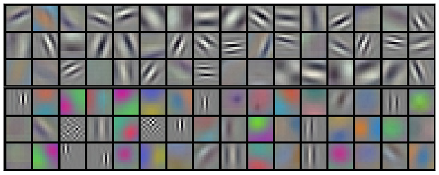
\includegraphics[width=0.9\textwidth]{figures/gabor_filters.png}
	\caption{set of Gabor filters \cite{gabor_filters}}
	\label{fig:set of Gabor filters}
\end{figure}

Straturile convoluționale au doi parametri pe care le putem modifica pentru a obține modificarea comportamentului fiecărui strat. După ce am ales dimensiunile stratului, trebuie să alegem \textit{stride} și \textit{padding}. \newline
Stride controlează cum filtrul convoluțional se mișcă pe suprafața matricii de pixeli a imaginii de intrare. \newline
De exemplu dacă $stride=1$ atunci filtrul este mișcat du pași de un pixel. De obicei valoarea parametrului stride se alege astfel încât imaginea generată de filtrul convoluțional să aibă dimensiuni de numere întregi nu fracții. Să luăm un exemplu: să ne imaginăm o imagine de intrare a carei dimensiune este 7x7 pixeli, și un filtru convoluțional de dimensiunea 3x3 cu un stride de un pixel.

%convolutional layer stride illustration
\begin{figure}[h!]
    	\centering
	\captionsetup{justification=centering, margin=2cm}
	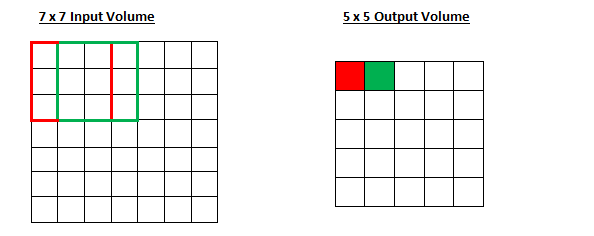
\includegraphics[width=0.9\textwidth]{figures/con_lay_stride.png}
	\caption{set of Gabor filters \cite{conv_lay_params}}
	\label{fig:con_lay_str}
\end{figure}


Pe figura\ref{fig:con_lay_str} putem vedea că matricea rezultată a valorilor produse de stratul convoluțional are dimensiunea de 5x5. Dar ce s-ar întâmpla dacă am folosi un stride de 2 pixeli? În acest caz pe axa orizontală putem să plasăm filtrul în trei poziții, la fel și pe axa verticală. Deci dimensiunile ieșirii filtrului are fi 3x3.\newline
Putem vedea că cu un stride mai mare ieșirea filtrului se micșorează. Putem observa și faptul că dacă stride ar fi trei, atunci am avea probleme cu plasarea filtrului. De obicei valoarea lui stride este mai mare decât unu dacă vrem ca regiunile receptive să nu se suprapună.\newline
Să aruncăm o privire și pe parametrul numit \textit{padding}. Înainte de a intra în detalii despre acest parameru, să cedem o situație reală: ce s-ar întâmpla dacă am aplica un filtru de 5x5 pe o imagine de 32x32? Dimensiunile ieșirii ar fi 28x28, deci imaginea se micșorează. Aplicând mai multe filtre convoluționale consecutive pe o imagine, ne lovim de o problemă: dimensiunile imaginii se reduc mai repede decât am dori. În primele straturi a rețelei neuronale dorim să conservăm cât mai multă informație.\newline
Să zicem că vrem să aplicăm același filtru convoluțional pe același imagine, dar de data asta ne folosim și de un padding, și anume: \textit{zero-padding}. Acesta înseamnă că mărim imaginea originală cu 2 pixeli in fiecare dimensiune, astfel ajungând la dimensiunea de 36x36. Elementelor nou-introduse în matrice le asignăm valoarea de 0.\newline
Ce am realizat cu introducerea paddingului este că după aplicarea aceluiași filtru (dimensiunea de 5x5 pixeli cu stride=1) imaginea rezultată nu mai este micșorată, ci rezultatul tot o să fie de 32x32.\newline
Formula pentru a calcula dimensiunile ieșirii pentru un strat convoluțional este
\begin{equation}
	O = \frac{W-K+2P}{S}+1
\end{equation}
unde K este dimensiunea filtrului, W este dimensiunea imaginii de intrare, P este valoarea paddingului și S este stride.


\subsection{Straturi nonlineare (Nonlinearity Layers)}
Aceste straturi acționează ca filtre nonlineare: intrarea este o matrice sau o imagine, peste care se aplică o activare \textit{non-saturating}. Pot fi de mai multe feluri:
\begin{itemize}
	\item ReLU: această funcție ia intrarea după ce aplică funcția de activare $f(x)=max(0, x)$. După ce a aplicat funcția de tranziție, propagă matricea sau imaginea rezultată mai departe,
	\item Tanh: această funcție ia intrarea și aplică funcția re activare $f(x)=tanh(x)$, după ce rezultatul este propagat mai departe,
	\item Sigmoid: acest tip de funcție ia intrarea peste care aplică funcția de tranziție $f(x)=exp(-x)+1$.
\end{itemize}

%non-linear activation functions
\begin{figure}[h!]
    	\centering
	\captionsetup{justification=centering, margin=2cm}
	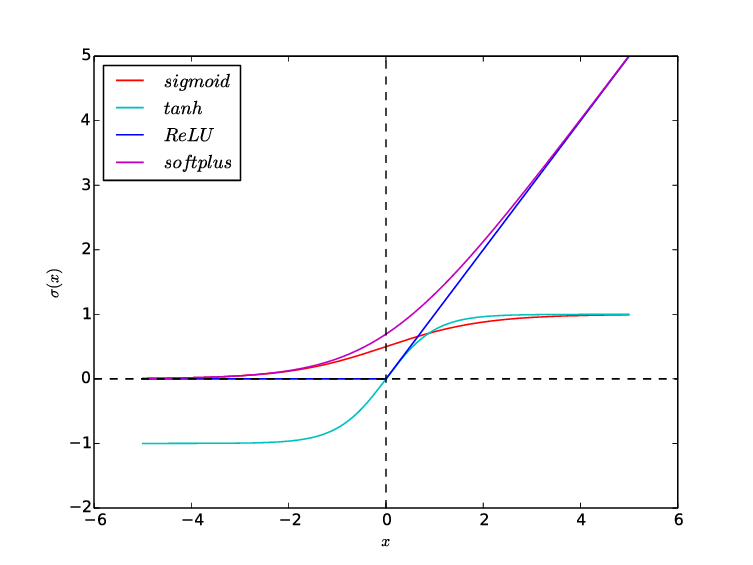
\includegraphics[width=0.9\textwidth]{figures/nonlinear_activation_functions.png}
	\caption{Funcțiile de transfer nonlineare \cite{non_lin_act_fun}}
	\label{fig:set of Gabor filters}
\end{figure}

\subsection{Local-Response Normalization Layers}
Acest tip de strat are ca intrare ieșirea de la stratul anterior și se folosește atunci când valorile de intrare pot fi infinit de mari. Acest strat normalizează într-un mod uniform intrările mari dintr-o regiune. Astfel face posibil ca activările foarte puternice să competizeze în grupuri de neuroni.

\subsection{Pooling Layers}
Acest tip de strat este specific rețelelor neuronale convoluționale; impune un \textit{downsampling} nonlinear a ieșirilor din stratul precedent. Există mai multe tipuri, cum ar fi max-pooling, average pooling, L2-norm pooling.\newline
Max-pooling este metoda cea mai des folosită, și funcționează în următorul fel: ca intrare se primeste o matrice sau o imagine. Această matrice sau imagine este partiționată în regiuni care nu se suprapun, regiunile având mărime bine definită. Din fiecare regiune se propagă mai departe numai cea mai puternică activare/cel mai puternic semnal. Acest fenomen are semnificația următoare: dacă într-o regiune am găsit a trăsătură fominantă, atunci poziția exactă a trăsăturii nu contează; este important numai să știm poziția relativă a acestei trăsături față de celelalte trăsături dominante.\newline
Beneficiul acestui tip de strat este acea că se reduce mărimea imaginii, extragându-se numai trăsăturile cele mai importante din ea. Ca urmare, după un strat pooling, numărul parametrilor rețelei se micșorează seminficativ fiindcă cantitatea informației din imagine se micșorează și ea. Astfel numărul ponderilor este redus drastic (75\%) reducând timpul și efortul de computație. Un alt beneficiu introdus de acest tip de strat este să controlează și \textbf{overfitting}ul. Overfitting este fenomenul prin care un model (o rețea neuronală) nu face generalizările necesare despre entitățile pe care trebuie să le recunoască, ci extrage și învațâ trăsături specifice din exemplele de antrenare. Principala simptomă a unei rețele care face overfitting este că pe setul de antrenare are o eficiență de peste 90\% dar numai 50\% pe setul de imagini de testare.

%max-pooling layer
\begin{figure}[h!]
    	\centering
	\captionsetup{justification=centering, margin=2cm}
	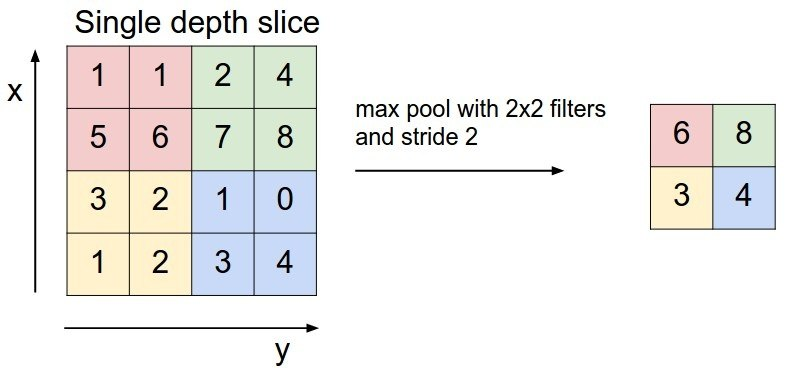
\includegraphics[width=0.9\textwidth]{figures/max_pol.jpg}
	\caption{Stratul max-pooling \cite{max_pol}}
	\label{fig:Stratul max-pooling }
\end{figure}

\subsection{Fully-Connected Layers}
Într-o rețea neuronală convoluțională, acest tip de strat execută sarcina predicției la nivel înalt. Se numește fully-connected pentru că neuronii din acest strat sunt interconectați cu fiecare neuron de pe stratul precedent.\newline
Activările stratului fully-connected pot fi calculate cu o simplă înmulțire între matrici (intre matricea de intrări și matricea de ponderi) și aplicând matricea de deplasare.

\subsection{Dropout Layer}
Acest tip de strat este prezent în rețelele neuronale convoluționale pentru a previne fenomenul de \textit{overfitting}. După antrenarea rețelei neuronale cu ajutorul setului de antrenare, scopul nostru este atingerea unei performanțe cât mai înalte pe setul de testare. Pentru a evita \textit{overfitting} și a induce un nivel mai mare de generalizare, straturile dropout fac următorul: iau neuroni cu probabilitate de $p=0.5$, pentru a fi scoase temporal din rețea. Muchiile de intrare și ieșire sunt scoase până la sfârșitul iterației.\newline
Astfel rețeaua neuronală are mai puține parametri în fiecare iterație, forțându-l să generalizeze în loc de overfitting. La sfârșitul fiecărei iterații neuronii eliminați sunt reintroduși în rețea cu ponderile neschimbate.

%dropout layer
\begin{figure}[h!]
    	\centering
	\captionsetup{justification=centering, margin=2cm}
	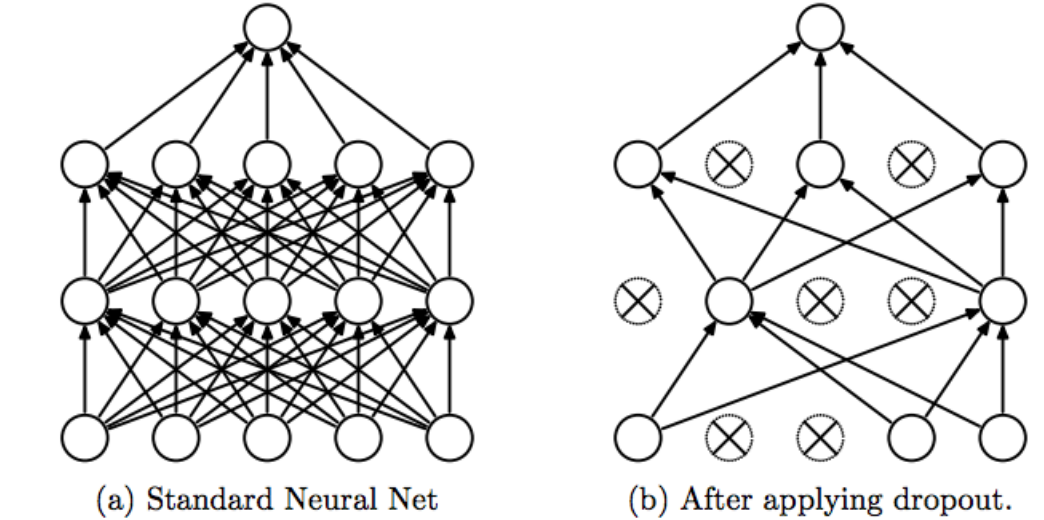
\includegraphics[width=0.9\textwidth]{figures/dro_out_lay.png}
	\caption{Drop-out layer \cite{dro_out_lay}}
	\label{fig:drop-out layer}
\end{figure}

\subsection{Softmax layer}
Ultimul strat dintr-o rețea neuronală convoluțională este un \textit{loss layer} folosing abordarea softmax.\newline
Acest strat are responsabilitatea de a calcula deviația dintre predicția rețelei și realitate (valoarea expectată). 


\label{cap:fund-teoretice}